\documentclass[12pt, letterpaper]{article}
\usepackage[utf8]{inputenc}
\usepackage{graphicx}
\graphicspath{ {.} }
\usepackage{wrapfig}
\usepackage{subfig}
 
\title{ASTP-720 Assignment 3}
\author{Brendan Drachler}
\date{\today}

\begin{document}

\section*{Problem 1}

My ODE solver library is located in ODE\_solver.py.

\section*{Problem 2}

We can use scipy's odeint function to solve the coupled differential equations that govern the motion of a pendulum. The equations are of the form:

\begin{equation}
\frac{d \theta(t)}{dt} = \Omega(t)
\end{equation}
\begin{equation}
\frac{d \Omega(t)}{dt} = -b \ \Omega(t) - c \sin(\theta(t))
\end{equation}

Odeint gives the following solution:

\includegraphics{{odeint_pendulum}.png}

Now, we can use the ODE library I wrote to solve the same set of equations as a validation tool for the solvers.

\newpage

\begin{figure}[ht]
\centering
\begin{tabular}{ccc}
\includegraphics[width=50mm]{{euler_pendulum}.png} &   \includegraphics[width=50mm]{{heuns_pendulum}.png} &  \includegraphics[width=50mm]{{rk4_pendulum}.png} \\
\end{tabular}
\end{figure}


Qualitatively, they look like they've done a great job! But it is more useful to compute the error between the solutions. The absolute error between our rk4 solution and the odeint output is: 

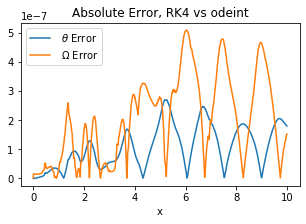
\includegraphics{RK4_vs_odeint.png}

The maximum error is of the order $5 \times 10^{-7}$. This is good enough to validate our numerical solvers!

\section*{Problem 3}

Now, we will try to solve a stiff ODE of the form: 

\begin{equation}
\frac{dy(t)}{dt} = -\lambda (y(t) - \cos(t))
\end{equation}

Subject to the initial condition: 

\begin{equation}
y(0) = 0
\end{equation}

We will compare our numerical solution to the analytical solution that takes the form:

\begin{equation}
y(t) = -\frac{\lambda^2}{1 + \lambda^2} e^{-\lambda t} + \frac{\lambda}{1 + \lambda^2} \sin(t) + \frac{\lambda^2}{1 + \lambda^2} \cos(t)
\end{equation}

I've tried solving the ODE for values of $\lambda$ ranging from 1 to 100 but my numerical solvers all struggle with it. I've also seen various online resources that claim stiff ODEs can sometimes be solved with explicit methods if the timestep is sufficiently small. Therefore, I've tried varying $dx$ from $0.01$ to $10^{-8}$ but still cannot solve this ODE. 

My numerical solvers are able to "hang on" for a little, but eventually diverge from the solution. All 3 solvers struggle with this function and no particular scheme seems to do better than the rest.

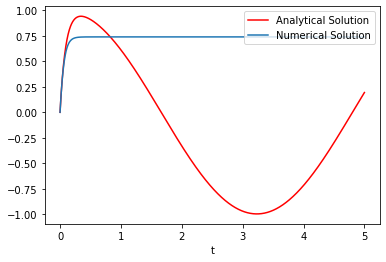
\includegraphics{stiff_EQ_Failure.png}

\newpage

\section*{Problem 4}
I used my RK4 solver to solve the coupled ODEs governing hydrostatic equilibrium in white dwarfs. The mass-radius relationship I found for WDs is:

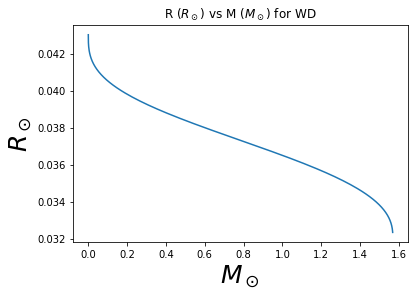
\includegraphics{WD_R_vs_M.png}

This is comparable to many of the plots in the literature that analyze the mass-radius relationship of WDs. The one noticeable difference is that my solution goes slightly beyond $ R \approx 1.4$. My solution actually does extend to $R = 0$ but I've only plotted this region because the region between $0 < R < 0.32$ is a vertical line that would wash out the features in this portion of the plot.

\section*{Problem 5}
I used my RK4 solver to solve the coupled ODEs governing hydrostatic equilibrium in neutron stars. The mass-radius relationship I found for NSs
is:

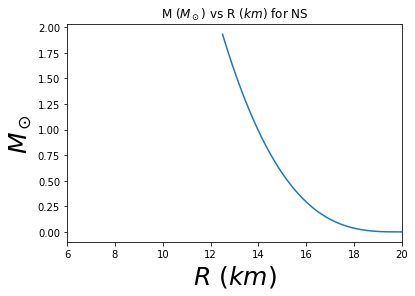
\includegraphics{NS_M_vs_R.png}

I chose the limits of the x-axis to mimic a very popular plot that I've seen in the literature many times (found here: https://arxiv.org/pdf/1205.6871.pdf):

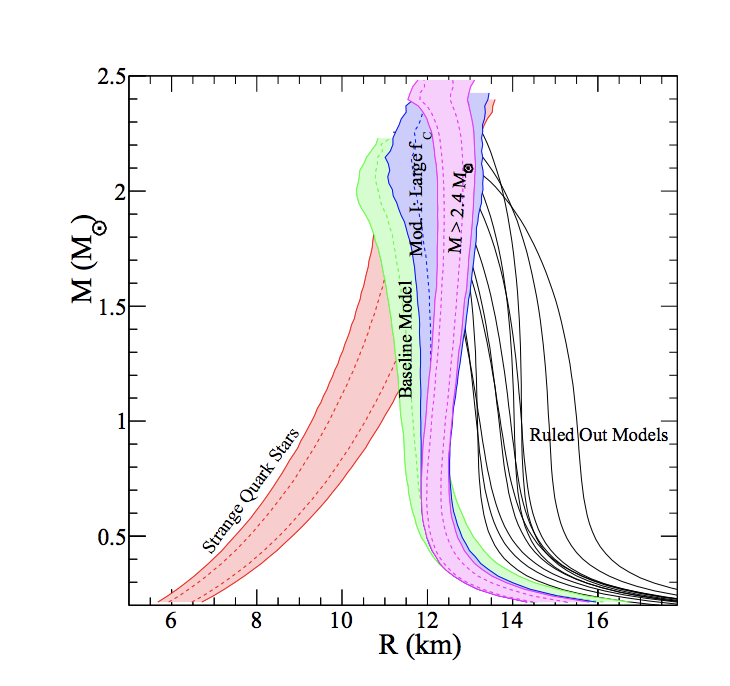
\includegraphics{NS_lit.png}

My solution matches up with many of the EOS in the literature. Though, I think it falls in the "ruled-out" region. 


\end{document}